\chapter{クラスの例}
この回はクラスの例を示す。
\section{例の概要}
図\ref{color}はここで示す例の表示画面である。
\begin{figure}[ht]
 \begin{center}
  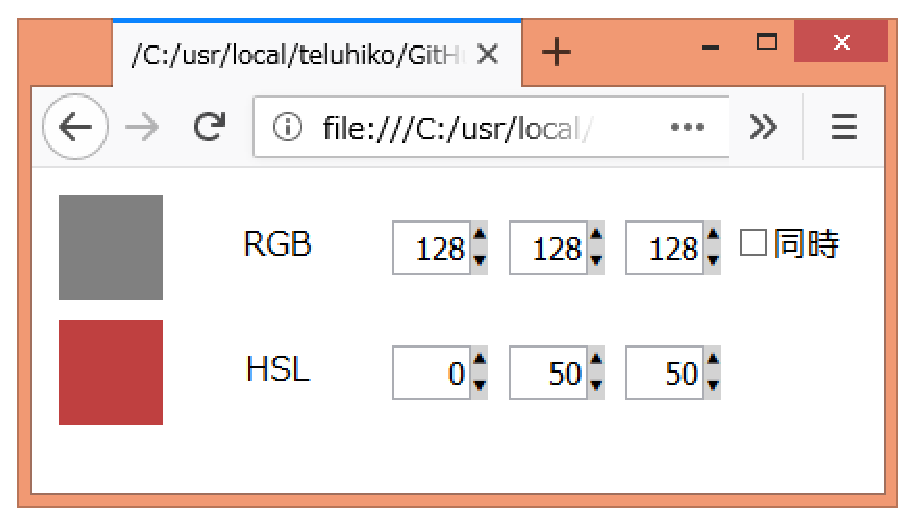
\includegraphics[width=0.5\textwidth]{13Ex.eps}
 \end{center}
 \caption{色の指定を見る}\label{color}
\end{figure}

この例では上下2行のテキストボックスで指定された色を左側の正方形の部分で
示す。上はRGB形式で、下はHSL\footnote{W3CのCSS Color Module Level
3\texttt{https://www.w3.org/TR/2011/REC-css3-color-20110607/}を参照のこ
と}形式で色を指定することができる。色を変える操作は次のとおりである。
\begin{itemize}
 \item それぞれのテキストボックスの値は▲をクリックすると増加し、▼をクリッ
       クすると1ずつ減少する。シフトキーを押しながらクリックすると5ずつ
       変化する。
 \item RGB形式の値は$0\sim255$の間で変化する。上限または下限の範囲を超え
       る場合は上限または下限の値にのままである。一番右のチェックボックスを
       チェックすると3つの値が同時に増減する。
 \item HSL形式の値は一番左(H--色相)が$0\sim359$の間で循環して変化し、残
       りの2つは$0\sim100$の間で変化する。
\end{itemize}
\section{ソースコードの解説}
\subsection{HTMLファイル}
次のリストはHTMLファイルのものである。
\LISTN{13Ex.html}{1}{last}{\small}
\begin{itemize}
 \item 5行目ではこのページに関する処理を定義する\JS ファイル
       (\texttt{13Ex.js})を読み込む。
 \item 6行目ではユーザーインターフェイスを定義している\JS ファイル
       (\texttt{13UI.js})を読み込む。
 \item 7行目から15行目は色を表示する部分のCSSを定義している。
       \begin{itemize}
        \item 9行目と10行目では表示部分の大きさ
        \item 11行目では配置方法(横に並べる)
        \item 12行目では上下の位置(ここでは中央に指定)
        \item 13行目では色の表示域の周りの空白
       \end{itemize}
 \item 18行目と19行目では色の表示位置と値を設定するための\texttt{<div>}
       要素を定義している。
\end{itemize}
 \section{ユーザーインターフェイス}
 次のリストはユーザーインターフェイスのクラスを定義するものである。

次のリストの部分は指定されたオブジェクトに指定できるオプションの値を変更するた
 めの関数を定義している。
 \LISTN{13UI.js}{1}{5}{\small}
\begin{itemize}
 \item 2番目の引数(\texttt{Opt})は変更する値が入っているオブジェクトであ
       る。
 \item 1番目の引数はキーがオブジェクト内の指定できるオプション(デフォル
       ト値が設定されている)からなるオブジェクトである。
 \item 3行目で指定できるキーであれば値を設定している。
\end{itemize}
次のリストの部分はHTML要素に対する\texttt{style}を設定するための関数である。
\LISTN{13UI.js}{6}{10}{\small}
\begin{itemize}
 \item 7行目で、指定されたオプションを設定している。
 \item 9行目でオプションのオブジェことを\texttt{style}属性の形式になるよ
       うに変更している。
\begin{enumerate}
 \item オブジェクトを\texttt{JSON}形式の文字列に変換
 \item キーなどを囲む\texttt{\{}と\texttt{\"}を取り除く
 \item \texttt{,}と\texttt{\}}を\texttt{;}に変換
\end{enumerate}
\end{itemize}
11行目から43行目のリストの部分は基本となるオブジェクト\texttt{DOMObject}を定義
している。
\LISTN{13UI.js}{11}{43}{\small}
\begin{itemize}
 \item オブジェクト内で有効な定数を定義するためにクラス式を返す関数を定
       義しその場で実行している(43行目の\texttt{()})。
 \item 12行目から15行目で作成する要素の名前空間のリストをオブジェクトリ
       テラルの形で定義している。ここではHTML要素とSVG要素の名前空間があ
       る。
 \item 17行目から19行目で\texttt{document.getElementById()}の相当する
       このオブジェクト用の関数を定義している。
 \item 20行目から24行目で\texttt{document.getElementsByTagName()}の相当する
       このオブジェクト用の関数を定義している。
       \begin{itemize}
        \item 21行目で指定された要素のリストを得ている。
        \item 22行目から23行目でそのリストを\texttt{DOMObject}のリストに
              変更している。
        \item \ElmJ{map}は配列オブジェクト\ElmJ{Array}のメソッドで、各要
              素に対して引数で与えられた関数を実行し、その結果からなる配
              列を返す。
        \item 21行目で得られたリストは配列ではないのでこのメソッドを使用
              できない。
        \item \ElmJ{call}は指定した関数が参照する\ElmJ{this}をその1番目
              の引数にする。
        \item 23行目の\texttt{(E)}以降の書き方は新しい無名関数の
              記述方法である。
\begin{Verbatim}
  function(E){...}
\end{Verbatim}
              と書くのと同じである。
        \item 新しい書き方と従来の書き方の一番の違いは関数内での
              \ElmJ{this}の取り扱いである。\ElmJ{class}内のコードは
              \texttt{strict}モードで実行される。このとき、
              \ElmJ{function}で定義された関数内では\ElmJ{this}は
              \ElmJ{undefined}になる。一方、簡略化された記述では
              \ElmJ{this}の値がオブジェクト自身を指す。この違いが問題と
              なる例はこのリストの170行目などにある。
       \end{itemize}
 \item 25行目から43行目はこのオブジェクトの\ElmJ{constructor}を定義して
       いる。
       \begin{itemize}
        \item 引数は順に作成する要素名、その属性のリスト、親要素、イベン
              ト処理のリスト、名前空間(デフォルトはHTML)である。
        \item 27行目で名前空間を指定して要素を作成している。
        \item 28行目は作成した要素に、与えられた属性を設定する関数を呼び
              出している。
        \item 29行目から31行目では親要素がある場合にはその子要素になるよ
              うに指定している。
        \item 32行目から34行目ではイベント処理を設定している。
        \item 37行目から42行目では与えられたリストの属性を設定する関数を
              定義している。
       \end{itemize}
\end{itemize}
次のリストの部分は与えられた文字列を表示するためのクラス\texttt{divWithText}を
定義している。
\LISTN{13UI.js}{44}{49}{\small}
\begin{itemize}
 \item このクラスは\texttt{DOMObject}を継承している。
 \item コンストラクタの引数は順に、表示するテキスト、親要素、属性である。
 \item 46行目で\texttt{<div>}要素を作成し、その要素の\ElmJ{innerText}プロパティを
       設定することで表示を可能としている
\end{itemize}
次のリストの部分は与えられた文字列を表示し、そのあとにテキストボックスを
表示するためのクラス\texttt{NamedTextBox}を定義している。
\LISTN{13UI.js}{50}{58}{\small}
\begin{itemize}
 \item このクラスは\texttt{divWithText}を継承している。
 \item コンストラクタの引数は順に、表示するテキスト、親要素、テキストボックス
       の大きさとその初期値である(51行目)。
 \item 作成した\texttt{<div>}要素の子要素にテキストボックスを作成してい
       る(53行目から55行目)。
 \item 57行目でテキストボックスの値を読み出すゲッター\texttt{value}を定
       義している。
\end{itemize}
次のリストの部分はボタンクラスを作成するものである。
\LISTN{13UI.js}{59}{65}{\small}
\begin{itemize}
 \item このクラスは\texttt{divWithText}を継承している。
 \item コンストラクタの引数は順に、ボタンに表示するテキスト、親要素、ボ
       タンのイベント処理関数のリストである(60行目)。
 \item 61行目で親要素の設定を行っている。
 \item 62行目でボタン要素を付け加えている。
\end{itemize}
66行目からのリストの部分はテキストボックスに付属した値を上下するボタンを持つ
\texttt{spinbox}のクラスを定義している。HTMLにも\texttt{spinbox}があるが
少し機能を変えている。

次のリストはこのクラスのコンストラクタの部分である。
\LISTN{13UI.js}{66}{98}{\small}
\begin{itemize}
 \item コンストラクタの引数は順に、オプション、親要素、イベント処理関数
       群、値が変化したときの処理関数である。
 \item 68行目は値が変化したときに呼び出される関数をオブジェクトに登録し
       ている。
 \item 69行目から73行目ではこのオブジェクトのデフォルトのパラメータを定
       義している。
       \begin{itemize}
        \item \texttt{max}は設定できる値の最大値(デフォルト値は
              JavaScriptで扱うことができる最大値)
        \item \texttt{mix}は設定できる値の最小値(デフォルト値は
              JavaScriptで扱うことができる最小値)
        \item \texttt{skip}は値の変化量(デフォルト値は$1$)
        \item \texttt{bigSkip}はシフトキーを押しながらクリックしたときの
              値の変化量(デフォルト値は$5$)
        \item \texttt{value}は初期値(デフォルト値は$0$)
        \item \texttt{type}は両端の値から外れたときの処理方法(デフォルト
              は両端の値に固定--\texttt{\"limited\"}。値が循環的に変わる
              \texttt{\"cyclic\"}がある)
       \end{itemize}
 \item 74行目から75行目でオブジェクトの周りの余白の設定をしている。
 \item 76行目で入れ物の\texttt{<div>}要素を作成している。
 \item 77行目では69行目からのデフォルトのパラメータを与えられた値に変更
       している。
 \item 78行目から79行目では81行目から83行目で定義されるテキストボックス
       を入れるための\texttt{<div>}要素を作成している。
 \item 81行目から83行目で定義されるテキストボックスは値を直接変更できな
       い設定をしている(\texttt{\"readonly\"}の指定)
 \item 84行目から85行目ではテキストボックスの隣に置く上下のボタンを入れ
       るための\texttt{<div>}要素を作成している。
 \item 86行目から89行目では値の上下させるボタンの表示形式を定義している。
 \item 90行目でさらにボタンのタイプ(値を増加)を設定し、91行目から92行目でボタンと
       して機能するようなオブジェクトを追加している。この上でクリックイ
       ベントが生じたときにイベント発生時ののシフトキーの状態を
       \texttt{sipnbox}の\texttt{up}プロパティの与えている(代入で行って
       いるが、\texttt{up}は101行目から110行目で定義されているセッターで
       ある)。
 \item 94行目から97行目は値を減少させるボタンを設定している。
\end{itemize}
残りの部分はこのクラスのセッターまたはゲッターを定義している部分である。
\LISTN{13UI.js}{99}{121}{\small}
\begin{itemize}
 \item 99行目と100行目はそれぞれテキストボックスの値に関するゲッ
       ターとセッターである。
 \item 101行目から110行目は設定値を増大させるメソッドであり、11行目から
       121行目は設定値を減少させるメソッドである。
 \item 102行目ではシフトキーが押されているかを判定して、変化量を決めてい
       る。
 \item 103行目で仮の値を求め、それが上限値を超えている処理を
       \texttt{spinbox}の\texttt{type}に応じて変えている(104行目から108
       行目)。
 \item  上限値で固定(\texttt{type}が\texttt{\"limited\"})のときは
       上限値と仮の値の小さい方を設定している(107行目)。
 \item 値gが循環する(\texttt{type}が\texttt{\"cyclic\"})ときは
       上限値が超えた場合、最小値を設定している(108行目)。
 \item 値の設定後の処理関数が定義されているときはその関数を呼び出す(109
       行目)。
 \item 値が減少する場合も同様である。
\end{itemize}
\LISTN{13UI.js}{122}{last}{\small}
 \section{ユーザーインターフェイスを引用するJavaScriptファイル}
 次のリストはユーザーインターフェイスを利用して、色の変化を見えるように
 するものである。
 \LISTN{13Ex.js}{1}{last}{\small}
 